\documentclass[border=3pt]{standalone}
% Preâmbulo compartilhado pelos diagramas TikZ da aula 7 de IHR (Emoção)
\usepackage[T1]{fontenc}
\usepackage[utf8]{inputenc}
\usepackage{lmodern}
\usepackage{amsmath}
\usepackage{xcolor}
\usepackage{tikz}
\usetikzlibrary{arrows.meta,angles,quotes,decorations.pathmorphing,decorations.pathreplacing,calc,
                positioning,shapes.geometric,shapes.misc,backgrounds,fit,
                math}

% Paleta (mesma dos SVGs originais)
% Paleta da disciplina de IHR: acento azul (#1A6FB5), cor de destaque do tema.
% (o nome "dblue" é mantido para não alterar todos os diagramas)
\definecolor{dblue}{HTML}{1A6FB5}
\definecolor{dorange}{HTML}{B3541E}
\definecolor{dgreen}{HTML}{4A7C59}
\definecolor{dred}{HTML}{9C4B4B}
\definecolor{dcream}{HTML}{F4F1EA}
\definecolor{dshade}{HTML}{DDD7C9}

% Função gaussiana (não normalizada por padrão de escala visual)
\pgfmathdeclarefunction{gauss}{3}{%
  \pgfmathparse{1/(#3*sqrt(2*pi))*exp(-((#1-#2)^2)/(2*#3^2))}%
}

% Estilos comuns (prefixo d... para não colidir com chaves internas do pgf)
\tikzset{
  >={Stealth[length=2mm]},
  dguide/.style={gray!55, dashed, line width=0.4pt},
  daxis/.style={gray!60, line width=0.7pt, ->},
  dbody/.style={fill=black!3, draw=black!80, line width=1pt},
  dacc/.style={draw=dblue, line width=1pt},
  dlbl/.style={black!55, font=\small},
  dsub/.style={black!45, font=\footnotesize},
  dstate/.style={circle, draw=black!80, fill=dcream, line width=1pt,
                 minimum size=17mm, font=\large, inner sep=1pt},
  dobs/.style={circle, draw=black!80, fill=dshade, line width=1pt,
               minimum size=14mm, font=\large, inner sep=1pt},
  dbox/.style={rounded corners=2pt, draw=black!80, fill=dcream, line width=1pt,
               align=center, inner sep=6pt},
  dop/.style={circle, draw=black!80, fill=white, line width=1pt,
              minimum size=6mm, inner sep=0pt, font=\small},
  dtrans/.style={->, dblue, line width=1pt},
  dmeas/.style={->, dorange, line width=1pt},
  dcurve/.style={line width=1pt, dblue},
  dcurveb/.style={line width=1.4pt, dorange},
}

\begin{document}
\hyphenpenalty=10000 \exhyphenpenalty=10000 \tolerance=9999 \emergencystretch=3em
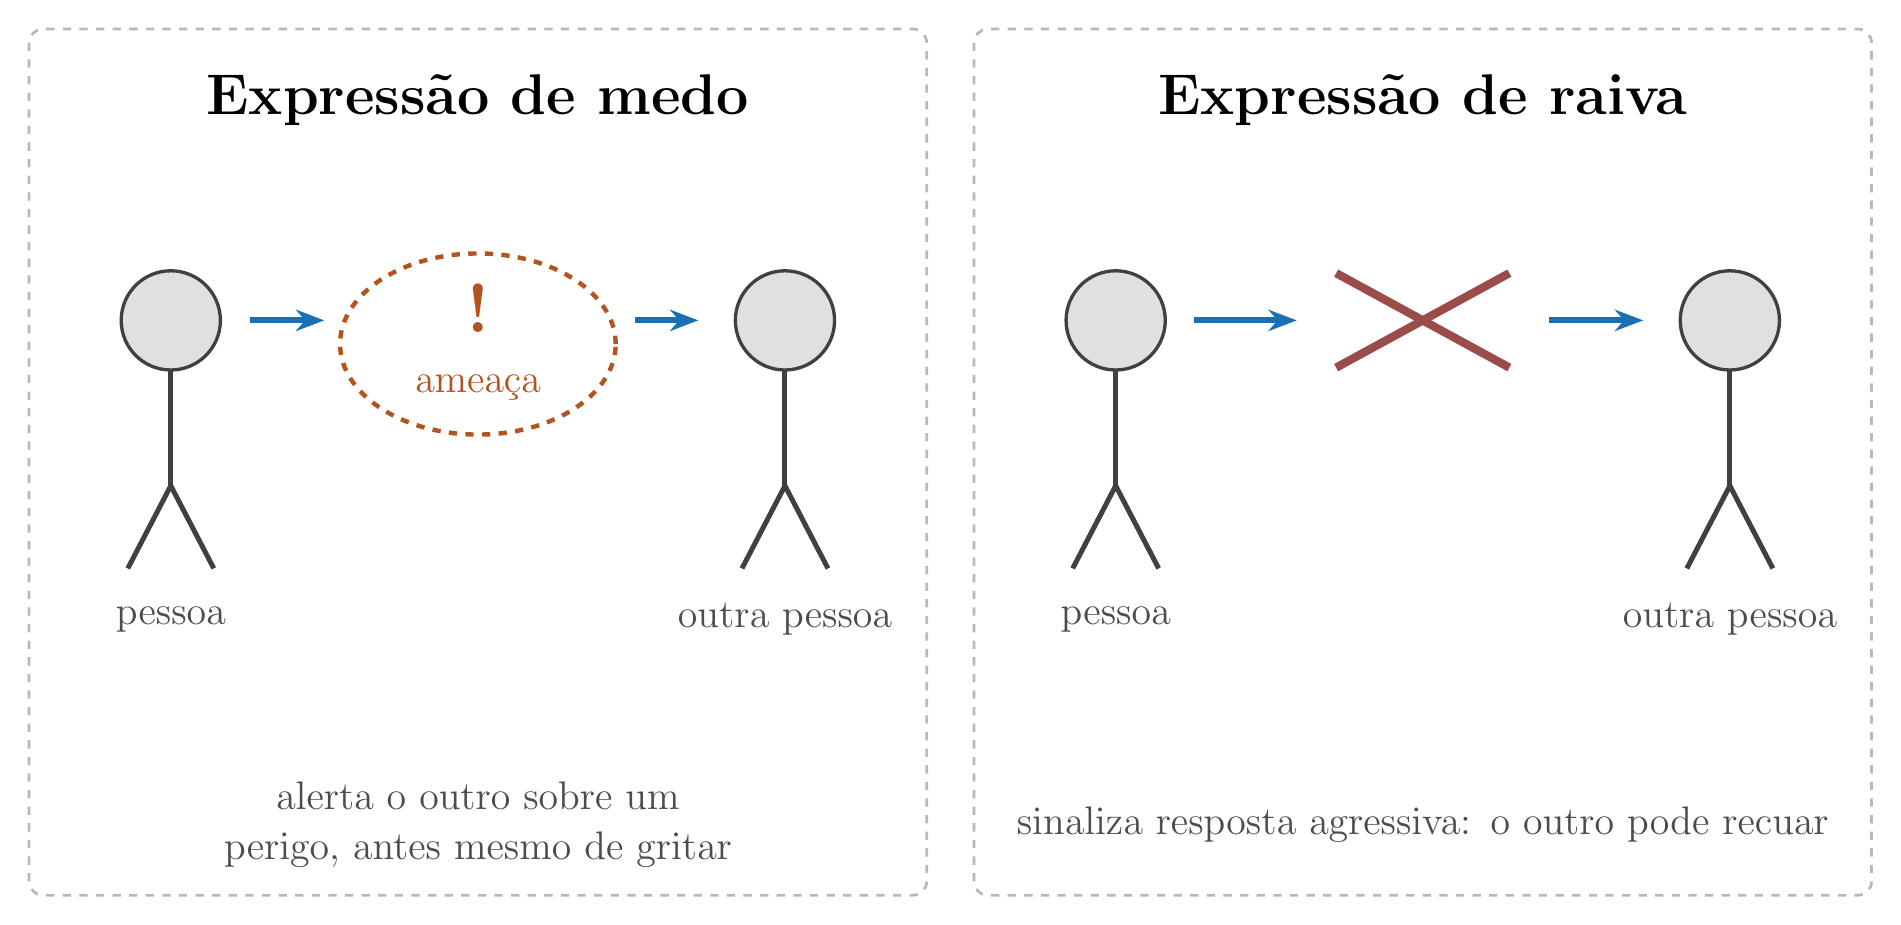
\begin{tikzpicture}[x=1cm,y=1cm]
  \newcommand{\perso}[3]{\begin{scope}[shift={(#1,#2)}, scale=2.1]
      \fill[black!12, draw=black!75, line width=1.2pt] (0,0) circle (0.30);
      \draw[black!75, line width=1.8pt] (0,-0.30) -- (0,-1.0);
      \draw[black!75, line width=1.8pt] (0,-1.0) -- (-0.26,-1.5);
      \draw[black!75, line width=1.8pt] (0,-1.0) -- (0.26,-1.5);
      \end{scope}
      \node[font=\Large, black!70] at (#1,#2-3.8) {#3};}

  % Medo
  \begin{scope}[shift={(0,0)}]
    \draw[dguide, rounded corners=5pt, line width=1pt] (-1.4,-5.3) rectangle (10.0,5.7);
    \node[font=\huge\bfseries] at (4.3,4.8) {Expressão de medo};
    \perso{0.4}{2.0}{pessoa};
    \draw[dguide, rounded corners=2pt, draw=dorange, line width=1.6pt] (4.3,1.7) ellipse (1.75 and 1.15);
    \node[dorange, font=\Huge\bfseries] at (4.3,2.15) {!};
    \node[font=\Large, dorange] at (4.3,1.15) {ameaça};
    \perso{8.2}{2.0}{outra pessoa};
    \draw[dtrans, line width=2.2pt, -{Stealth[length=3.6mm]}] (1.4,2.0) -- (2.35,2.0);
    \draw[dtrans, line width=2.2pt, -{Stealth[length=3.6mm]}] (6.3,2.0) -- (7.1,2.0);
    \node[font=\Large, align=center, black!70, text width=10.4cm] at (4.3,-4.4) {alerta o outro sobre um perigo, antes mesmo de gritar};
  \end{scope}

  % Raiva
  \begin{scope}[shift={(12.0,0)}]
    \draw[dguide, rounded corners=5pt, line width=1pt] (-1.4,-5.3) rectangle (10.0,5.7);
    \node[font=\huge\bfseries] at (4.3,4.8) {Expressão de raiva};
    \perso{0.4}{2.0}{pessoa};
    \draw[dred, line width=3pt] (3.2,2.6) -- (5.4,1.4);
    \draw[dred, line width=3pt] (5.4,2.6) -- (3.2,1.4);
    \perso{8.2}{2.0}{outra pessoa};
    \draw[dtrans, line width=2.2pt, -{Stealth[length=3.6mm]}] (1.4,2.0) -- (2.7,2.0);
    \draw[dtrans, line width=2.2pt, -{Stealth[length=3.6mm]}] (5.9,2.0) -- (7.1,2.0);
    \node[font=\Large, align=center, black!70, text width=10.4cm] at (4.3,-4.4) {sinaliza resposta agressiva: o outro pode recuar};
  \end{scope}

\end{tikzpicture}
\end{document}
